\documentclass[11pt]{article}
\usepackage{geometry}
\usepackage{graphicx}
\usepackage{enumitem}
\usepackage{float}

\geometry{a4paper, top=0.5in, bottom=0.5in, right=0.75in, left=0.75in}

\title{Static Timing Analysis}
\author{Abanoub Emad Hanna}
\date{}

\begin{document}

\maketitle

\section*{Timing Definitions}
    \textbf{Contamination Delay:} Output may begin to change or glitch.\\
    \textbf{Propagation Delay:} Output must have settled to final value. \\
    \textbf{Setup Time:} The time the input data signals are stable before the active clock edge occurs (D to CLK). \\
    \textbf{Hold Time:} The time the input data signals are stable after the active clock edge occurs (CLK to D). \\
    \textbf{Aperture Time:} Setup time + hold time \\
    \textbf{Sequencing Overhead:} $t_{pcq}+t_{setup}+t_{skew}$ \\
    \textbf{Recovery Time:} The reset/set signal has to return to its normal state before the clock edge for this duration, similar to the setup time.\\
    \textbf{Removal Time:} The reset/set signal has to remain in the reset/set state after the clock edge for this duration, similar to the hold time.\\

    \begin{center}
        \centering
        \vspace{-20pt}
        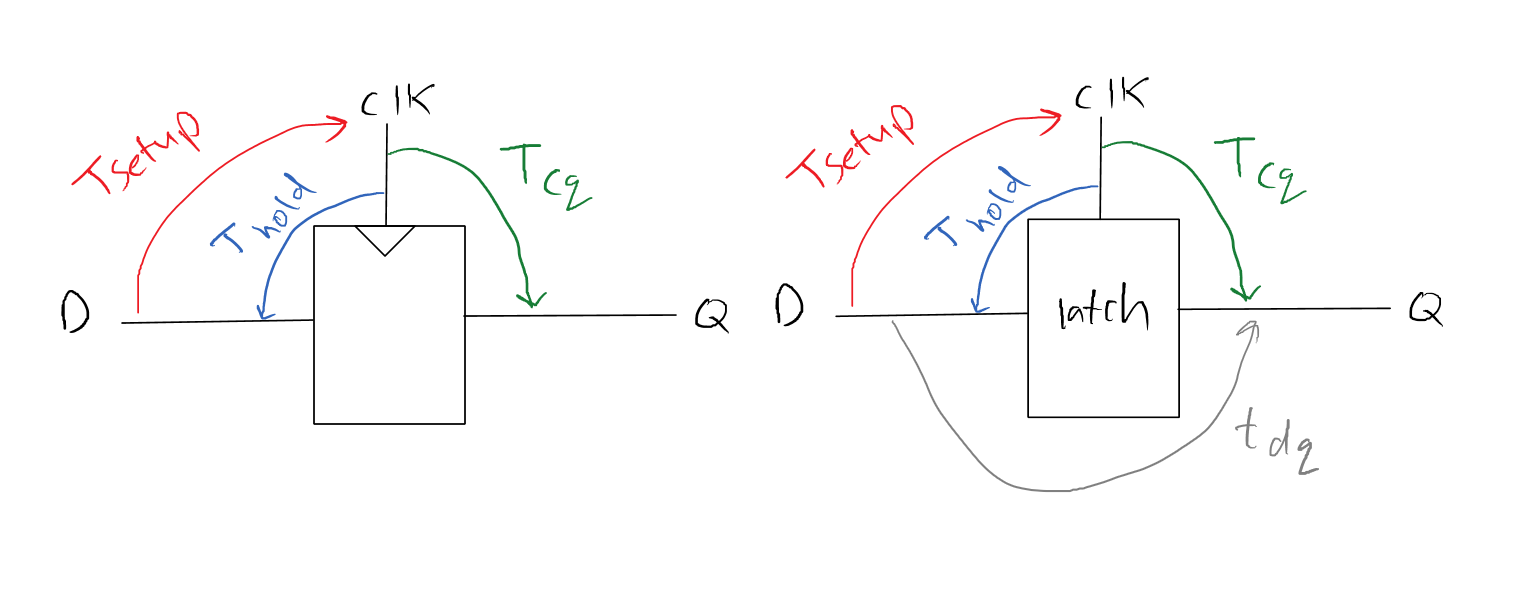
\includegraphics[scale=0.5]{1}
        \vspace{-40pt}
    \end{center}
    \textbf{Notes:}
    \begin{itemize}
        \item Tcq is useful when Q is CLK-sensitive like in FF (all cases) or in latch (when D is constant and latch toggles from opaque to transparent).
        \item We can achieve negative hold time by delaying the input (D). We can achieve a smaller setup time by delaying the CLK.
        \item The smaller the $t_s$, $t_h$ and $T_c$, the bettter.
        \item $t_{cq}$ can be different for the same FF cell due to different load capacitance.
    \end{itemize}
    
    \begin{center}
        \centering
        \vspace{-10pt}
        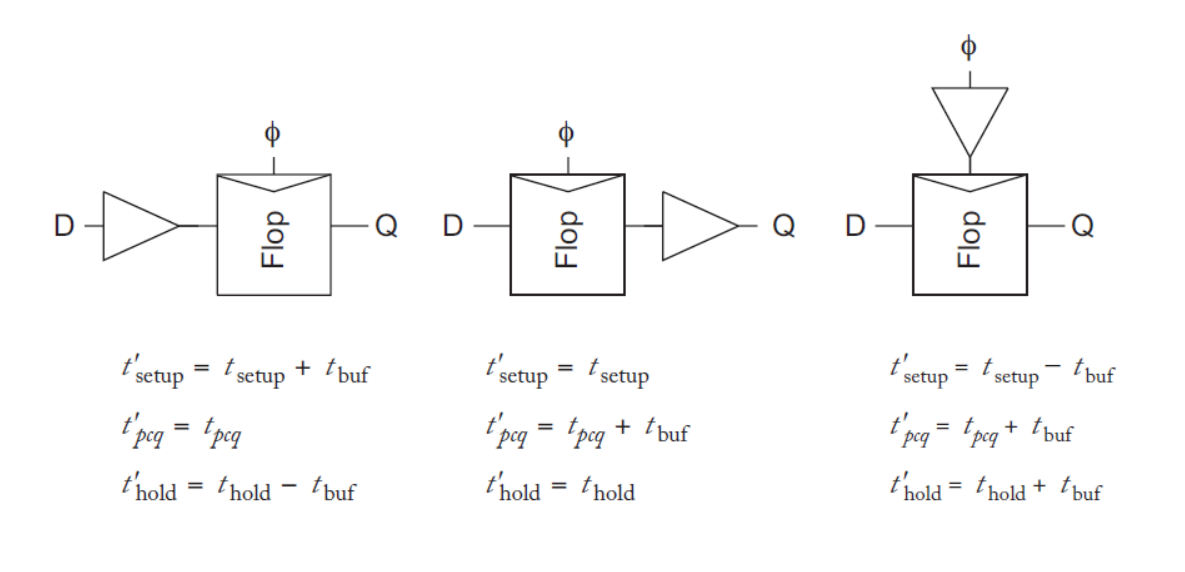
\includegraphics[scale=0.5]{2}
    \end{center}
    \newpage

\section*{Timing Analysis}
    \textbf{Note: } We measure clock period from a point to the same exact point in the next cycle (i.e, from CLK to CLK (same edge: -ve to -ve or +ve to +ve) or D to D).\\ \\
    \textbf{Clock Skew \& Jitter:} 
    \begin{itemize}
        \item \textbf{Clock Skew:} Spatial variation across chip
        \begin{itemize}
            \item \textbf{Positive Skew:} 
            \begin{itemize}
                \item CLK's edge of FF2 is later than FF1. 
                \item CLK drivers are in the same direction as the combinational logic.
                \item Difference between 2 CLK edges is increased.
                \item Bad for hold time, since data must be preserved for a longer time (waiting for the delayed FF2's CLK edge).
            \end{itemize}
            \item \textbf{Negative Skew:}
            \begin{itemize}
                \item CLK's edge of FF2 is earlier than FF1. 
                \item CLK drivers are in the opposite direction as the combinational logic.
                \item Difference between 2 CLK edges is reduced.
                \item Bad for setup time, since actual clock period is reduced for a given clock frequency.
            \end{itemize}
        \end{itemize}
        \item \textbf{Clock Jitter:} Temporal variation at the same element (random)
        \begin{itemize}
            \item \textbf{Worst case (setup): } When launching FF is late \& capturing FF is early. Actual clock period is reduced (for a given frequency).
            \item \textbf{Worst case (hold): } When launching FF is early \& capturing FF is late. Data is held for a longer time.
        \end{itemize}
    \end{itemize}
    \textbf{Max-delay constraints:}
    \begin{itemize}
        \item Maximum propagation delay (data didn't settle before CLK edge)
        \item Setup time failure
        \item $T_c + t_{skew}> T_{pcq} + t_{pd} + t_s$ ($t_{skew}$ is a negative number for worst case)
    \end{itemize}
    \textbf{Min-delay constraints:}
    \begin{itemize}
        \item Minimum contamination delay (early change of data after CLK edge or data is so fast that it passes through
        several FFs during the same clock cycle.)
        \item Hold time failure (race condition)
        \item $t_h + t_{skew} < t_{ccq} + t_{cd}$ ($t_{skew}$ is a positive number for worst case)
    \end{itemize}
    \textbf{Note:} 
    \begin{itemize}
        \item In synthesis tool, we set input delay constraint from launching FF's CLK to the design block's input. The output delay is set from the design block's output to the capturing FF's CLK.
        \item Slack = Required time - Arrival time. 
        \begin{itemize}
            \item \textbf{Setup:} slack = $(T_{clk} - t_{setup}) - (T_{pcq} + t_{pd})$
            \item \textbf{Hold:} slack = $(T_{ccq} + t_{cd}) - T_{hold}$.
        \end{itemize} 
    \end{itemize}

\section*{Extra: Latch-Based Systems}
    \begin{center}
        \centering
        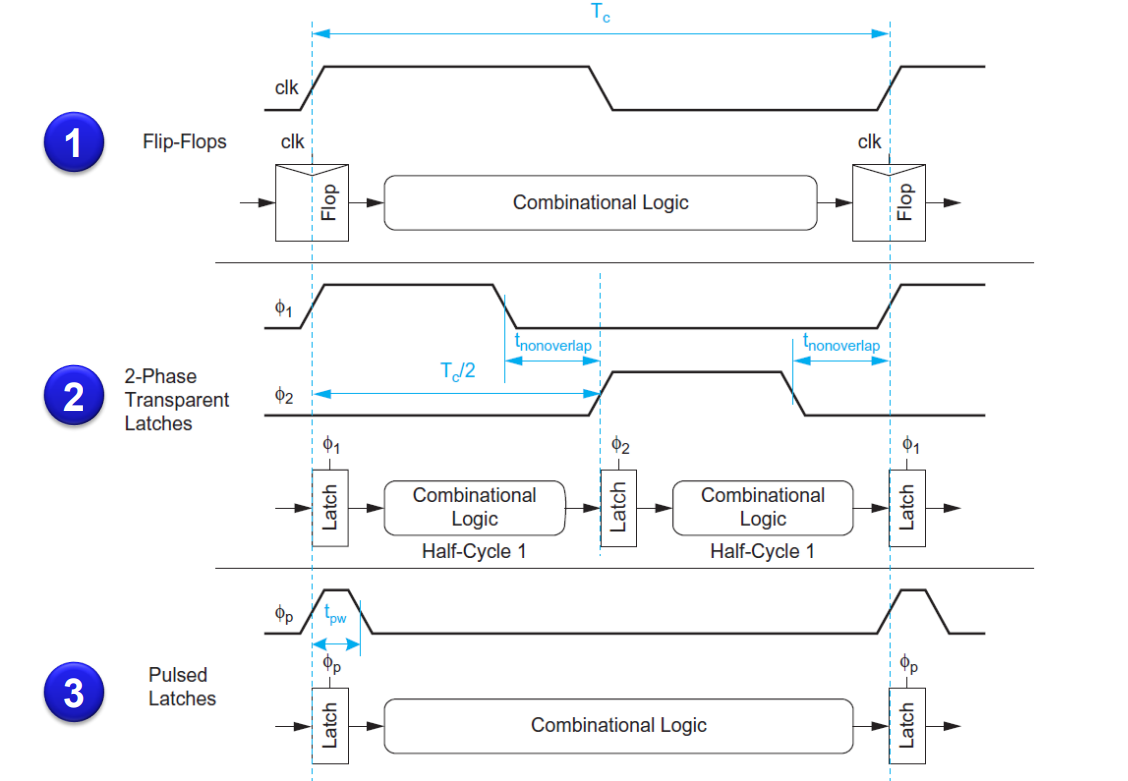
\includegraphics[scale=0.6]{3}
    \end{center}
    Maximum delay is given by:
    \vspace{5pt}
    \begin{itemize}[topsep=0pt]
        \item \textbf{2-phase transparent latch:} $T_c > T_{pdq1} + t_{pd1} + T_{pdq2} + t_{pd2}$ 
        \item \textbf{Pulsed Latch (D changes during pulse):} $T_c > T_{pdq} + t_{pd}$ ($t_{pw} > t_s$)
        \item \textbf{Pulsed Latch (D constant during pulse):} $T_c > T_{pcq} + t_{pd} + t_s - t_{pw}$ (from +ve edge CLK) ($t_{pw} < t_s$)
    \end{itemize}
    Minimum delay is given by:
    \vspace{5pt}
    \begin{itemize}[topsep=0pt]
        \item \textbf{2-phase transparent latch:} $t_h < t_{ccq} + t_{cd} + t_{nonoverlap}$
        \item \textbf{Pulsed Latch:} $t_h + t_{pw} < t_{ccq} + t_{cd}$
        \item \textbf{Note:} No timing violation for min delay if hold time is negative.\\
    \end{itemize}
    \textbf{Time Borrowing:} \\
    Time borrowing is only valid when system is latch-based (not FF), because it is not edge-sensitive, so data can be late and will still pass when latch is transparent.
    \begin{itemize}
        \item Max borrowing time:
        \begin{itemize}[topsep=0pt]
            \item \textbf{2-phase latch:} $t_{borrow} < T_c / 2 - (t_s + t_{nonoverlap})$
            \item \textbf{Pulsed latch:} $t_{borrow} < t_{pw} - t_s$
        \end{itemize}
        \item Actual borrowing time:
        \vspace{5pt}
        \begin{itemize}[topsep=0pt]
            \item \textbf{2-phase latch:} $t_{borrow} = t_{pdq} + t_{pd} - T_c / 2$
            \item \textbf{Pulsed latch:} $t_{borrow} = t_{pdq} + t_{pd} - T_{pw}$
        \end{itemize}
    \end{itemize}
    \textbf{Clock Skew:} 
    \begin{itemize}
        \item \textbf{2-phase latch:} It reduces $t_{nonoverlap}$. 
        \item \textbf{Pulsed latch:} It reduces $t_{pw}$.
        \item Therefore, skew increases hold time and reduces borrowing time.
    \end{itemize}
\end{document}
